% PDF für den Vortrag kompilieren (pro animierten Klick eine Seite)
% Option [t]: Inhalte am oberen Folienrand ausrichten
\documentclass[t, ]{beamer} 

% PDF für Handout (eine Seite pro Folie)
%\documentclass[handout]{beamer} 

%%% Foliendesign
\usetheme{Madrid}

%%% Packages

% Mathematik:
\usepackage{amsmath}
\usepackage{amsthm}
\usepackage{listings}

% Umlaute tippen
\usepackage[utf8]{inputenc}

% Deutsche Übersetzungen und Wörterbuch für korrekte Silbentrennung
% \usepackage[ngerman]{babel}

% Blockweises auskommentieren mit \begin{comment}\end{comment}
\usepackage{verbatim}

% Grafiken 
\usepackage{graphicx} % Bilder einblenden
\usepackage{xcolor} % Farbnamen einbinden
\graphicspath{{bilder/}} % Es gibt ein Unterverzeichnis, wo alle Bilder liegen. Durch diesen Befehl muss man nicht jedes mal den Dateipfad angeben

\usepackage{tikz} % Grafiken erstellen
\usetikzlibrary{arrows,automata} % Zusätzliche Tikz-Module einbinden
\tikzset{>=stealth, shorten >= 1pt,auto,node distance=2cm,} % Tikz Einstellungen
\tikzstyle{initial}+=[initial text=]

%%% Informationen für Titelseite
\title{Z3 Tutorial}
\subtitle{Perlen der Logik}
\author{Timo Lobitz} 
\date{22.Juli 2024}

%%% Folien 
\begin{document}

%% Titelfolie	
\begin{frame}[plain, noframenumbering]
    \titlepage
\end{frame}
\begin{frame}{Introduction}
	\begin{enumerate}
		\item Smartphone company OnePluZ3 is about to launch their new flagship phone
		\item You are facing several issues that need to be solved ASAP
	\end{enumerate}
	
\end{frame}
\begin{frame}{Problem 1 - What to produce?}
	\begin{itemize}
		\item You can produce 3 different items
		\begin{itemize}
			\item Phone cases, chargers, and smartphones
		\end{itemize}
		\item Each take different amounts of resources to produce and generate a different amount of profit
		\item You have limited labor hours, machine hours and material available
	\end{itemize}
	
\end{frame}

\begin{frame}{Problem 1 - What to produce?}
	Resources available:
	\begin{itemize}
		\item 500 labor hours
		\item 800 machine hours
		\item 600 units of material
	\end{itemize}
	
	\begin{table}
		\centering
		\begin{tabular}{cccccc}
			Name &  Profit & Labor Hours & Machine Time & Raw Materials \\
			Phone Case &  10 & 3 & 3 & 4\\
			Phone Charger & 30  & 5  & 3 &2 \\
			Smartphone & 50  & 4 & 5 & 6\\
		\end{tabular}
		\label{tab:resource_cost}
	\end{table}
	
\end{frame}

\begin{frame}{Problem 1 - Formalization}
	This can be expressed as a linear programming problem.  
	\begin{align}
		\max f(x) = 10 * A + 30 * B + 50 * C \\
		\text{with contraints}\\
		3*A + 5*B+ 4*C <= 500 \\
		3*A + 3*B + 5*C <= 800 \\
		4*A + 2*B + 6*C <= 600 \\
		A>=0 \\
		B>=0 \\
		C>=0
	\end{align}
\end{frame}

\begin{frame}{Problem 2 - Dependency Chaos}
	As part of the production line, you need to manage different parts and chips that are used in different devices.
	\begin{figure}
		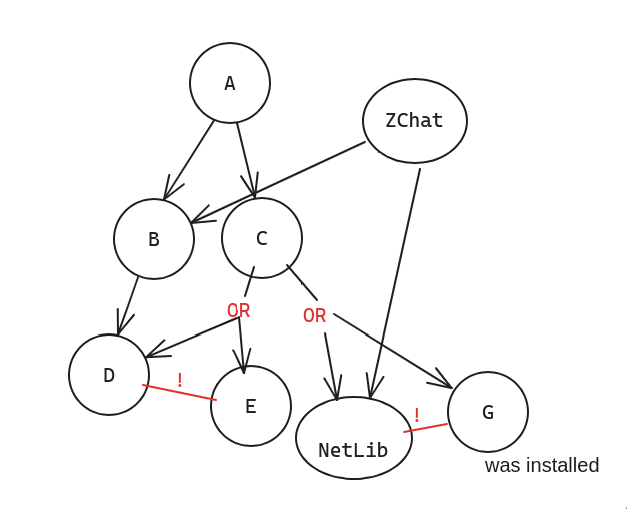
\includegraphics[scale=0.25]{../Images/deps.png}
	\end{figure}
\end{frame}

\begin{frame}{Problem 2 - Formalization}
	\begin{itemize}
		\item Each part is represented by a boolean variable
		\begin{itemize}
			\item True if in production
			\item False if not in production
		\end{itemize}
		\item A depends on B : $A \implies B$
		\item A conflicts with B : $\neg A \lor \neg B$
	\end{itemize}
\end{frame}



\begin{frame}{Problem 3 - Code Verification}
	The day 1 patch is currently in code review. You notice a strange function written by a coworker.
	\lstinputlisting[language=c]{magic.c}
\end{frame}


% Z3 Introduction
\begin{frame}{Z3}
	\begin{columns}
		\begin{column}{0.5\textwidth}
			\begin{itemize}
				\item SMT solver
				\item open-source
				\item from Microsoft Research
			\end{itemize}
		\end{column}
		\begin{column}{0.5\textwidth}
			\begin{figure}
				
\includegraphics[scale=0.3]{../Images/z3logo.png}
			\end{figure}
		\end{column}
		
	\end{columns}
	
\end{frame}

\begin{frame}{Z3}
	\begin{figure}
		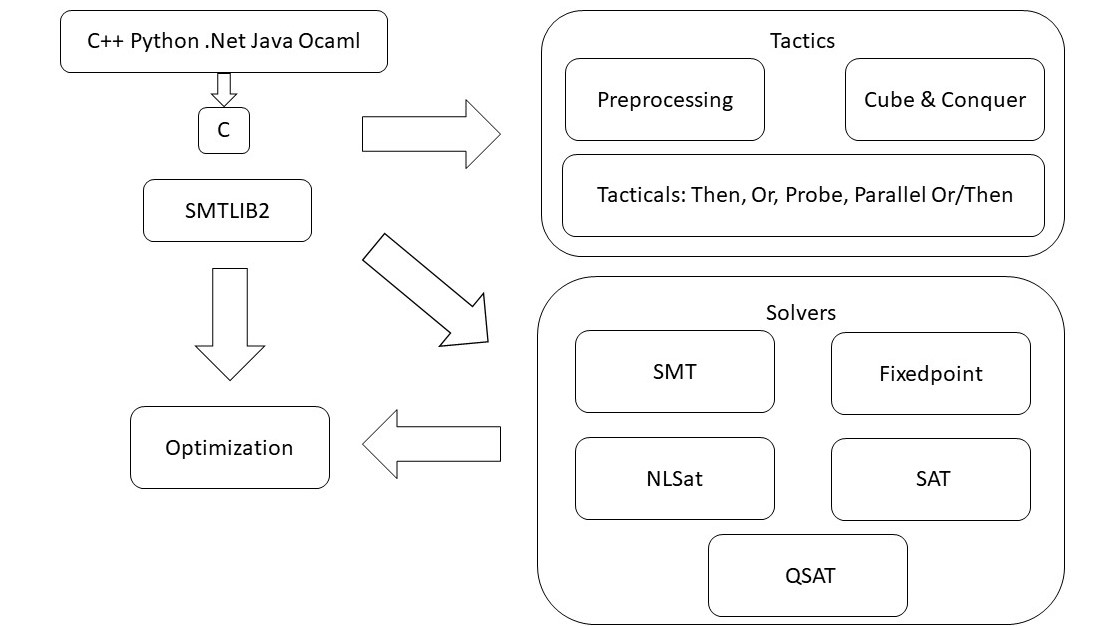
\includegraphics[scale=0.4]{z3intern.jpg}
	\end{figure}
\end{frame}

\begin{frame}{Z3 - Usage}
	
	
	\begin{columns}
		\begin{column}{0.4\textwidth}
			4 Step pattern:
			\begin{enumerate}
				\item Create Solver
				\item Define variables
				\item Add constraints
				\item Check
			\end{enumerate}
		\end{column}
		\begin{column}{0.6\textwidth}
			\pause
			\lstinputlisting[language=python]{usage.py}
			
		\end{column}
		
	\end{columns}
\end{frame}


\begin{frame}{Variables}
	
	\begin{columns}
		\begin{column}{0.4\textwidth}
			\lstinputlisting[language=python]{variables.py}
		\end{column}
		\begin{column}{0.6\textwidth}
			\lstinputlisting[language=python]{variables2.py}
			
		\end{column}
		
	\end{columns}
	
	
\end{frame}

\begin{frame}{Arrays}
	Arrays in Z3 map from one datatype to another. They support Store and Select operations. Store retrurns a new Arrays and doesn't change the input array.
	\lstinputlisting[language=python]{arrays.py}
	
\end{frame}

\begin{frame}{Custom Datatypes - Enum}
	\lstinputlisting[language=python]{enum.py}
\end{frame}


\begin{frame}{Custom Datatypes - List}
	\lstinputlisting[language=python]{list.py}
\end{frame}


\begin{frame}{Conclusion}
	\begin{itemize}
		\item Z3 is versatile and can be applied to a lot of problems, such as 
		\begin{itemize}
			\item Software Verification / Static analysis
			\item Optimization problems
			\item Mathematical proofs
			\item ...
		\end{itemize}
		\item Z3 is an efficient general solver for SAT and SMT problems
		\item Z3 can be used to determine satisfiability, optimize or proof formulas
	\end{itemize}
\end{frame}


\begin{frame}{References}
	\begin{itemize}
		\item Programming Guide by Microsoft \href{https://z3prover.github.io/papers/programmingz3.html}{https://z3prover.github.io/papers/programmingz3.html}
		\item Python tutorial by Microsoft \href{https://microsoft.github.io/z3guide/programming/Z3\%20Python\%20-\%20Readonly/Introduction}{https://microsoft.github.io/z3guide/programming/Z3\%20Python\%20-\%20Readonly/Introduction} 
		\item Z3 - Github \href{https://github.com/Z3Prover/z3}{https://github.com/Z3Prover/z3}
		\item SAT-SMT by example \href{https://smt.st/SAT\_SMT\_by\_example.pdf}{https://smt.st/SAT\_SMT\_by\_example.pdf}
		\item Z3 API \href{https://z3prover.github.io/api/html/namespacez3py.html}{https://z3prover.github.io/api/html/namespacez3py.html}
		
	\end{itemize}
\end{frame}

\begin{frame}{Github}
	Notebooks used : \href{https://github.com/TimoLob/Z3-Tutorial}{https://github.com/TimoLob/Z3-Tutorial}
\end{frame}

\end{document}